\subsection{AJAX} % (fold)
\label{sub:ajax}

Since its beginnings, the Web has been document based.
This means that, when the visitor wants more information and clicks on a link, the browser would request and load another whole document.
Even in web applications, the browser would have to reload the full page to send any information from the user and update the page.

\begin{wrapfigure}{r}{0.5\textwidth}
  \centering
    
\includegraphics[width=0.48\textwidth]{logo-not-ajax}
  \caption[AJAX logo]{This is not the \idx{AJAX} logo you are looking for}
  \label{fig:ajax-logo}
\end{wrapfigure}

This turns out to be inefficient and overkill in most situations, since web applications do not need to reload the full page in every user interaction but only update a little amount of information.
To address this problem several solutions where developed, from frames to applets, but they were too cumbersome or foreign respect the basic web technologies.

In 1999, \idx{Microsoft} proposed and implemented in its \idx{Internet Explorer} a new \idx{ActiveX} control to asynchronously load new data from the server without need to reload the page.
Using \idx{JavaScript}, that data could be requested on demand once the page was loaded, and through callbacks the data could be processed and the user interface changed accordingly.

Later, the rest of the browsers vendors implemented a similar technology under the \idx{XMLHttpRequest} object.
As this was gradually introduced, web developers started using it but it did not become a popular approach until 2004, when several big web applications such as \idx{Gmail} were developed.

Then, the term \ida{AJAX} was coined \cite{AJAX} to designate the technologies involved in the process, though most of them can be replaced by others while maintaining the same spirit.
Seeing how useful it had become, the \ida{W3C} decided to standardize the \idx{XMLHttpRequest} object.

As depicted in Figure~\ref{fig:ajax-application-model}, this approach needs another layer of complexity in the client to handle the data and update the interface.
This \ida{AJAX} engine means that much more \idx{JavaScript} code in the client is needed.
Eventually, this enables the rise of heavy web applications running in the client, with a substantial codebase to maintain and support across several browsers.

\begin{figure}[htbp]
  \centering
    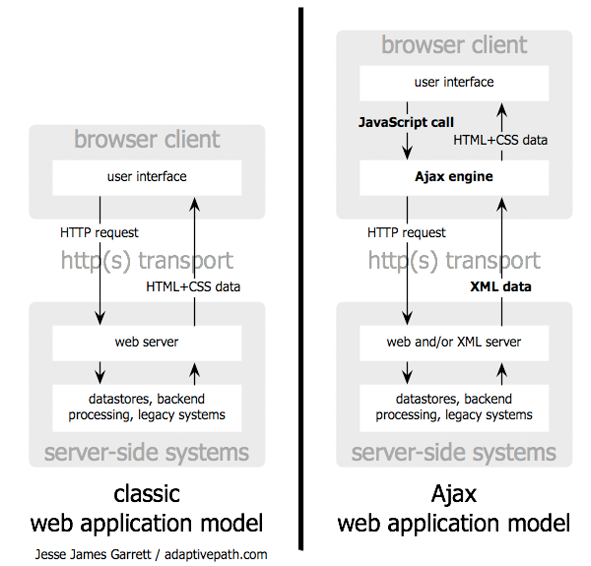
\includegraphics[width=\textwidth]{ajax-application-model}
  \caption[AJAX web application model]{AJAX web application model compared to the classic one.\newline© Jesse James Garrett}
  \label{fig:ajax-application-model}
\end{figure}

From the point of view of the user, the experience is much less disruptive than the classic model, as seen on Figure~\ref{fig:ajax-flow}.
When a user clicks a link or a button in a traditional web application, the user interface blocks, goes blank, and he has to wait until another page is fully reloaded if he wants to continue with another task.

\begin{figure}[htbp]
  \centering
    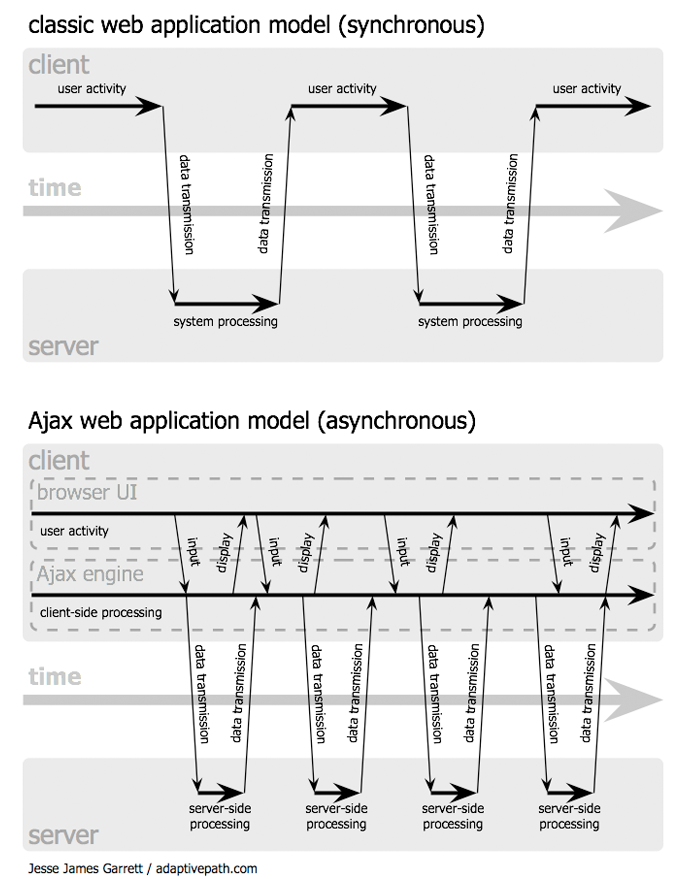
\includegraphics[width=\textwidth]{ajax-flow}
    \caption[AJAX flow]{Flow of the actions in a AJAX web application.\newline© Jesse James Garrett}
  \label{fig:ajax-flow}
\end{figure}

In an \idx{AJAX} application, when the user performs such actions, the interface does not block; instead the \idx{AJAX} engine is notified and the interface is \emph{instantly} available.
Meanwhile, backstage data gets interchanged and the client is updated, so that it can refresh the interface using the \ida{DOM} and a mix of \ida{HTML} and \ida{CSS}.

Though it could appear that the application has more overhead now, the user will notice a much more responsive application. Also, the requests should be much faster than before, since the browser does not need to process again all the resources or redraw the whole page, and the server only needs to generate fragments of data.

However, there are some drawbacks to this approach.
The first one is that the browser offers no feedback whatsoever to the user, but that is easily solved: the interface needs to reflect some visual feedback, like a spin ball.
The second one is that the application will break the history of the user, since no new page has been served, it cannot go back to the previous state or even link to it.
This has also been solved by the \ida{HTML}5 History \ida{API}, that allows to manipulate the browser history.

The third and hard one is that users with \idx{JavaScript} disabled will not be able to use this web application at all.
The best practice is to offer an alternate version with plain \ida{HTML} pages, but sometimes that is not possible or it makes no sense.
In the case of this project, since it was mostly experimental and not oriented for mainstream users, it was decided that such alternative would not be developed.

\subsubsection{How XMLHttpRequest works} % (fold)
\label{ssub:xmlhttprequest}

First of all, a \idx{XMLHttpRequest} object must be created, and a custom function that will be act as a callback must be set in its \texttt{onreadystatechange} property.
The next step consists of opening the connection to the server, with its \texttt{open()} method, specifying at least three parameters: first the \ida{HTTP} method to use (\texttt{"GET"} or \texttt{"POST"}), then the url that we wish to contact and finally if the requests should be asynchronous or not.
This last parameter is usually set to \texttt{true}, otherwise the user interface will block.

From now on, this object can make as many requests as it needs.
To make a request its \texttt{send()} method is used, with additional data if the method is \texttt{POST} or with no data (or \texttt{null}) if the method is \texttt{GET}.
Additionally, and only if needed, the \texttt{setRequestHeader()} method could be used to modify the headers of the \ida{HTTP} request.
If the request is asynchronous, the flow of the program will continue normally; if not, the program will block until the server sends all the data.

Some time later, the server will answer with the response data.
Then, the callback specified in the \texttt{onreadystatechange} property will be called, with all the needed data already updated in the \idx{XMLHttpRequest} object.
Actually, this callback will be called not only once but several times, each time reporting the progress of the request.
To be sure that the request was completed it is need to check that the \texttt{readyState} property is exactly 4, and to know that the requested resource is ok that the \texttt{status} property is 200 (this is the \ida{HTTP} state response).

If after that all was according to plan, the plain data will be accessible from the \texttt{reponseText} property.
Also, if the response is in \ida{XML}, the \texttt{reponseXML} property is also available with the parsed \ida{XML} tree (the reason of the X in \ida{AJAX}).
The callback will then usually make some \ida{DOM} manipulation to reflect the change in the interface.

Given the usefulness of this technique, most third-party libraries have implemented wrappers and more straightforward \ida{API}s to cover more use cases.
Also, there are different variations, for example the current trend is not to use the \ida{XML} format but to transmit everything in \ida{JSON}, a much more efficient markup language that is native to \idx{JavaScript}.

% subsubsection xmlhttprequest (end)

\subsubsection{JSONP} % (fold)
\label{ssub:jsonp}

By design, \idx{XMLHttpRequest} carries a severe restriction: it is only allowed to request \ida{URL}s from the same domain.
There are security reasons for this decision, but in this mashup golden era it hinders a lot of its purposes.
Thankfully, another technique has been popularized: \ida{JSONP}.
Less elegant than \ida{AJAX} but equally effective in most situations and without that ugly restriction.

The concept is simple and it is based on the fact that it is possible to add external scripts to a webpage.
Just add a \texttt{script} tag with the desired \ida{URL} and it will be executed; use the \ida{DOM} and that script can be dynamically added after the page is loaded, just like \ida{AJAX}.
Of course, that script must be written in \idx{JavaScript}, so that explains why  \ida{JSON} is used to pass the required data.

Listing~\ref{jsondata} shows how some data could be expressed in \ida{JSON} so that it can be used as an \ida{AJAX} response.
A question appears, how is that data going to be executed in order to access it?
The answer is by telling the external server to wrap it up in some function that we have define in our \idx{JavaScript} code.
The way to tell that to the other server is to add the name of the function to the requested \ida{URL} as a parameter (usually called \texttt{jsonCallback} or just \texttt{callback}).

\begin{lstlisting}[language=JavaScript,label=jsondata,caption=Some JSON data]
  {
    name:   "Kermit",
    animal: "Frog",
    age:    56,
    height: 45
  }
\end{lstlisting}

For example, if we tell the other server that the function is called \texttt{doSomethingWithData()}, it can then wrap it up in a way that the data is the parameter for that function (see Listing~\ref{jsonpdata}).
Since this code will be executed in our web application, it will call that function with that data at the exact moment the file is received and parsed.
Therefore, that function must be defined in the global object, so it can process the received data without any problem.

\begin{lstlisting}[language=JavaScript,label=jsonpdata,caption=Same JSON data wrapped in a custom function]
  doSomethingWithData({
    name:   "Kermit",
    animal: "Frog",
    age:    56,
    height: 45
  });
\end{lstlisting}

Obviously, the server must explicitly support this technique, otherwise it is impossible to receive and change the server response without the use of proxies.
Also, \ida{JSONP} should only be applied with trusted third parties, since any malicious code could be injected in the page.
The last security concern is that \texttt{POST} is not \emph{supported}, so any parameter has to be passed using \texttt{GET}, i.e., adding the parameters to the \ida{URL}.
However, due to its utility, almost all the popular libraries have similar tools that homogenizes  the use of \ida{AJAX} and \ida{JSONP}.

% subsubsection jsonp (end)

% subsection ajax (end)